\documentclass{beamer}
\usepackage{listings}
\usepackage{hyperref}
\usepackage{tikz}
\usetikzlibrary{positioning,shadows,arrows,shapes,calc}
\def\labelenumi\theenumi
\usepackage{graphicx}
\usepackage{xcolor}
\colorlet{ForestGreen}{green!50!black}
\usepackage{amsmath}
\mode<presentation>{\usetheme{Frankfurt}}
\AtBeginSection
{
  \begin{frame}<beamer>
    \frametitle{Outline}
    \tableofcontents[currentsection,currentsubsection]
  \end{frame}
}
\title{Lecture 23: Generative Adversarial Networks\\Reference: \href{http://papers.nips.cc/paper/5423-generative-adversarial-nets.pdf}{Goodfellow et al. (2014)}}
\author{Mark Hasegawa-Johnson\\All content~\href{https://creativecommons.org/licenses/by-sa/4.0/}{CC-SA 4.0} unless otherwise specified.}
\date{ECE 417: Multimedia Signal Processing, Fall 2020}  
\institute{University of Illinois}
\titlegraphic{\includegraphics{../../../17fall/lectures/imark_1867_bold.png}}
\begin{document}

% Title
\begin{frame}
  \maketitle
\end{frame}

% Title
\begin{frame}
  \tableofcontents
\end{frame}

%%%%%%%%%%%%%%%%%%%%%%%%%%%%%%%%%%%%%%%%%%%%%%%%%%%%%%%%%
\section{VAE vs.~GAN}
\setcounter{subsection}{1}

\begin{frame}
  \frametitle{VAE vs.~GAN}
  \begin{itemize}
  \item A {\bf VAE}
    \begin{itemize}
    \item scores $q(z|x)$  w.r.t. predefined prior $p(z)$,
    \item generates latent variables from $q(z|x)$,
    \item scores data using learned generator $p(x|z)$.
    \end{itemize}
  \item A {\bf GAN}
    \begin{itemize}
    \item generates latent variables from predefined prior, $p(z)$,
    \item generates data using learned generator $x=G(z)$,
    \item scores data using learned discriminator $D(x)$.
    \end{itemize}
  \end{itemize}
\end{frame}

\begin{frame}
  \frametitle{VAE vs.~GAN}

  \begin{itemize}
  \item {\bf Prior:} Same.  Both VAE and GAN assume a unit-normal Gaussian or uniform prior for $z$.
  \item {\bf Generator:} Similar.  GAN generates $x$ from $z$ using $x=G(z)$,
    therefore $x$ must be continuous.  VAE computes $p(x|z)$, so $x$
    could be either discrete or continuous.
  \item {\bf Scoring:} Very different.  VAE trains $q(z|x)$ to
    minimize $D_{KL}(p(z)\Vert q(z|x))$.  GAN trains $D(x)$ for no
    purpose other than scoring $x$.
  \end{itemize}
\end{frame}

\begin{frame}
  \frametitle{What is the discriminator?}

  \begin{itemize}
  \item The main innovation in GAN is the discriminator, $D(x)$.
  \item It outputs one number, $D(x)\in (0,1)$.
  \item If $x$ is good, $D(x)\rightarrow 1$
  \item If $x$ is bad, $D(x)\rightarrow 0$
  \end{itemize}
\end{frame}
  
\begin{frame}
  \frametitle{How can you train the discriminator?}

  The discriminator is trained by giving it 50\% real data, and
  50\% data generated synthetically by $G(x)$. Its training objective is:
  \begin{itemize}
  \item If $x$ is real data, the discriminator wants to output $D(x)\rightarrow 1$
  \item If $x$ is synthetic data generated by $G(z)$, the
    discriminator wants to output $D(x)\rightarrow 0$
  \end{itemize}
\end{frame}
  
%%%%%%%%%%%%%%%%%%%%%%%%%%%%%%%%%%%%%%%%%%%%%%%%%%%%%%%%%
\section[Probabilities]{Probabilistic interpretation of the GAN}
\setcounter{subsection}{1}

\begin{frame}
  \frametitle{Probabilistic interpretation of the discriminator}

  Let's say $y=1$ if a token is real data, $y=0$ if a token is fake data.
  The discriminator computes
  \begin{displaymath}
    D(x) = \Pr\left\{y=1|x\right\}
  \end{displaymath}
  Its goal is to maximize
  \begin{align*}
    V(D,G) 
    &= \mathbb{E}_{x\in\mbox{data}}\left[\ln \Pr\left\{y=1|x\right\}\right]
    +\mathbb{E}_{x\in\mbox{fake}}\left[\ln\Pr\left\{y=0|x\right\}\right]\\
    &= \mathbb{E}_{x\sim p_{data}}\left[\ln D(x)\right]
    +\mathbb{E}_{z\sim p(z)}\left[\ln\left(1-D(G(z))\right)\right]
  \end{align*}
\end{frame}

\begin{frame}
  \frametitle{Two-player minimax game}

  \begin{itemize}
  \item The discriminator wants to discriminate real vs.~fake data.
  \item The generator wants to make fake data that is as realistic as
    possible.  So its goal is to generate data, $x=G(z)$, in order to
    maximize $D(G(z))$.
  \item $D$ wants to maximize, and $G$ to minimize,
    \begin{displaymath}
      V(D,G)= \mathbb{E}_{x\sim p_{data}}\left[\ln D(x)\right]
      +\mathbb{E}_{z\sim p(z)}\left[\ln\left(1-D(G(z))\right)\right]
    \end{displaymath}
  \end{itemize}
\end{frame}

\begin{frame}
  \frametitle{The generator computes an implicit pdf, $p_g(x)$}

  \begin{itemize}
  \item The VAE explicitly computes $p(x|z)$.
  \item The GAN generates $z$ from $p(z)$, then generates $x=G(z)$.
    The resulting $x$ has some pdf, that you should be able to compute
    using ECE 313 methods if you wanted to.  Let's call this pdf
    $p_g(x)$.
  \item The goal of the generator might be phrased as follows: learn
    $G(x)$ so that $p_g(x)$ matches the true data distribution,
    $p_{data}(x)$, as well as possible.
  \end{itemize}
\end{frame}

\begin{frame}
  \frametitle{The training process for a GAN: $D(x)$, $p_{data}(x)$, and $p_g(x)$\\
    (c) Goodfellow et al., (2013), Figure 1}

  \centerline{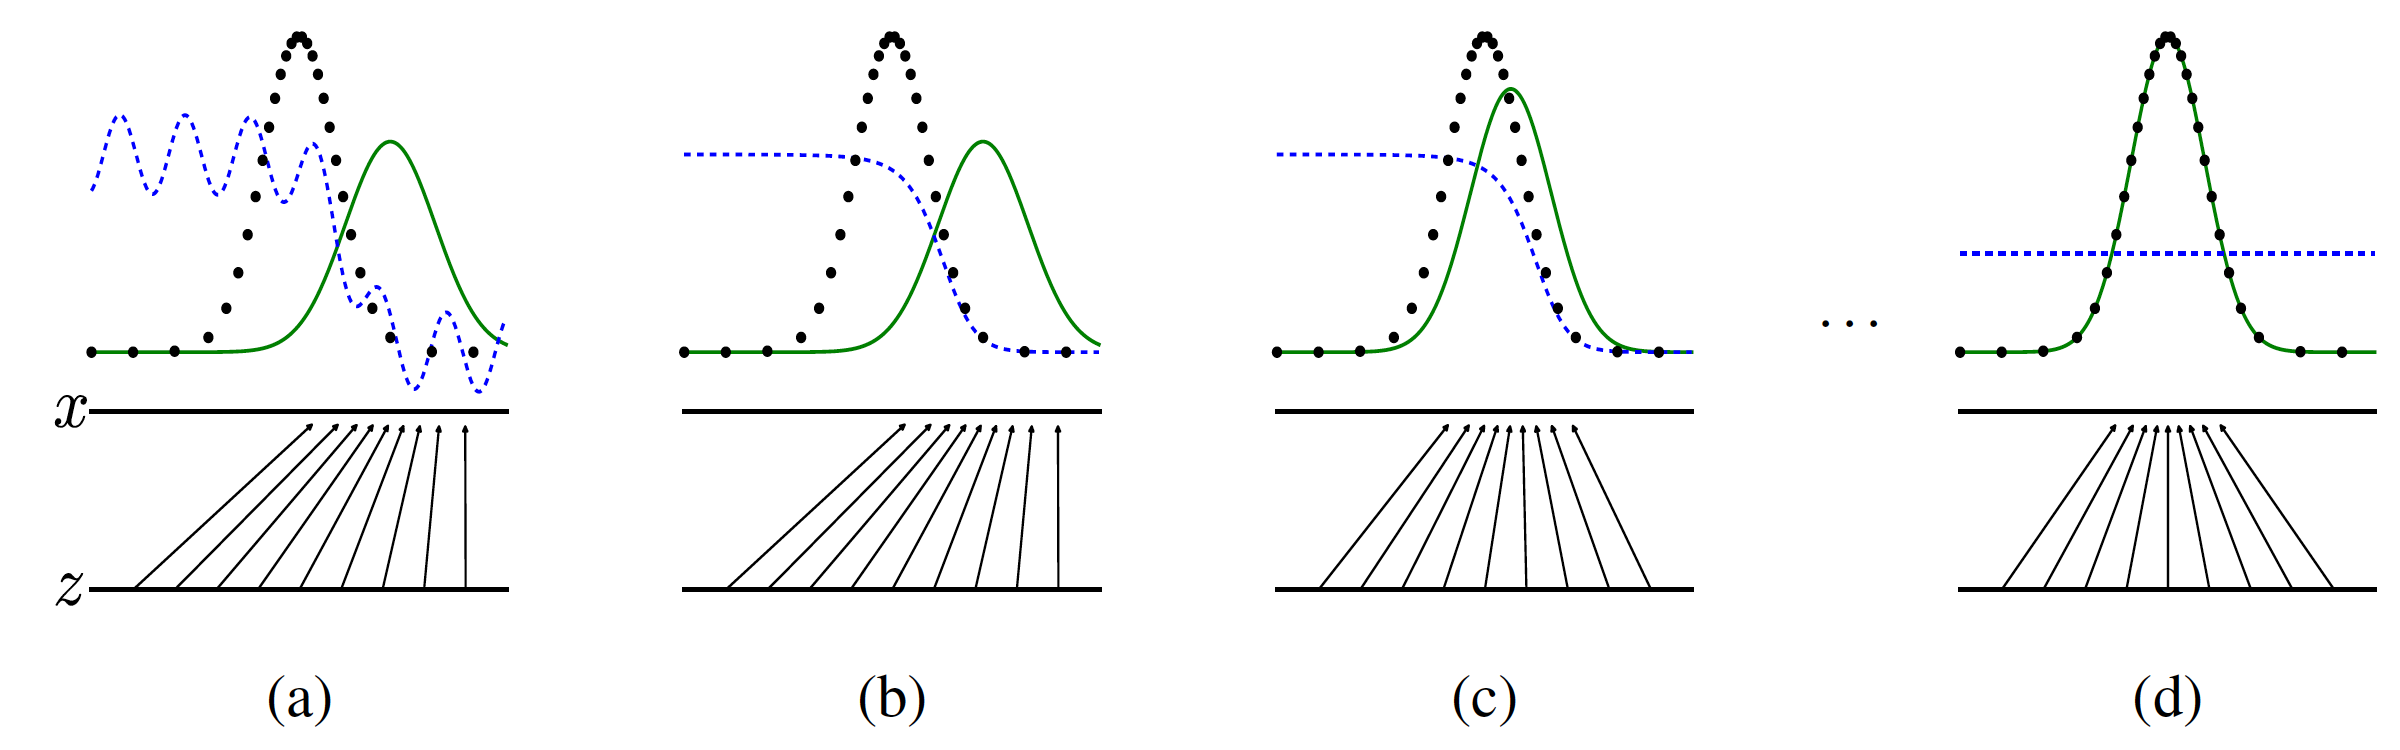
\includegraphics[width=4.5in]{goodfellow2014fig1.png}}
  \begin{itemize}
  \item {\color{blue}Blue small dots: $D(x)$}
  \item Black large dots: $p_{data}(x)$
  \item {\color{ForestGreen}Green solid: $p_g(x)$}
  \end{itemize}
\end{frame}

%%%%%%%%%%%%%%%%%%%%%%%%%%%%%%%%%%%%%%%%%%%%%%%%%%%%%%%%%
\section{Nash Equilibrium}
\setcounter{subsection}{1}

\begin{frame}
  \frametitle{Nash Equilibrium}

  \begin{itemize}
  \item Suppose two players, $D$ and $G$, are playing a game.
  \item Depending on their actions, they receive rewards $V_D(D,G)$
    and $V_G(D,G)$, respectively (in our case, $V_G=-V_D$, but that
    need not be true in general).
  \item Each of them has perfect knowledge about the other's actions:
    each knows, in advance, what the other will do.
  \end{itemize}
\end{frame}
  
\begin{frame}
  \frametitle{Nash Equilibrium}

  \begin{itemize}
  \item Player $D$ is called ``rational'' if, given knowledge of player G's action,
    their action is $D = \arg\max V_D(D,G)$.
  \item Player $G$ is called ``rational'' if, given knowledge of player D's action,
    their action is $G = \arg\max V_G(D,G)$.
  \item A {\bf Nash equilibrium} is a set of actions $(D,G)$ such
    that, each player knowing in advance the other player's action,
    neither player has any rational incentive to change.
  \end{itemize}
\end{frame}

\begin{frame}
  \frametitle{Nash Equilibrium for the GAN: Player $D$}

  First, suppose $G$ is known, therefore $p_G(x)$ is known.
  Now $D$ wants to maximize:
  \begin{align*}
    V(D,G) &= \mathbb{E}_{x\sim p_{data}}\left[\ln D(x)\right]
    +\mathbb{E}_{x\sim p_g}\left[\ln\left(1-D(x)\right)\right]\\
    &= \int \left(p_{data}(x)\ln D(x)+p_g(x)\ln\left(1-D(x)\right)\right)dx\\
    &= \int f(x)dx
  \end{align*}
  So for any particular $x$, the discrimator wants to maximize:
  \begin{displaymath}
    f(x)=p_{data}(x)\ln D(x)+p_g(x)\ln\left(1-D(x)\right)
  \end{displaymath}
\end{frame}
\begin{frame}
  \frametitle{Nash Equilibrium for the GAN: Player $D$}
  \begin{align*}
    f(x)&=p_{data}\ln D+p_g\ln\left(1-D\right)\\
    \frac{df}{dD} &= \frac{p_{data}}{D} - \frac{p_g}{1-D}\\
    \frac{d^2f}{dD^2} &= -\frac{p_{data}}{D^2} - \frac{p_g}{(1-D)^2}
  \end{align*}
  We find the maximizer by setting $df/dD=0$, which gives us
  \begin{displaymath}
    D^*_G(x) = \frac{p_{data}(x)}{p_{data}(x)+p_g(x)}
  \end{displaymath}
  Furthermore, we see that $f(x)$ is a convex function of $D$, and
  therefore $D^*_G(x)$ is the unique global maximizer, because
  \begin{displaymath}
    \frac{d^2f}{dD^2} < 0~~\forall D\in [0,1],~p_{data}>0,~p_g>0
  \end{displaymath}
\end{frame}

\begin{frame}
  \frametitle{Nash Equilibrium for the GAN: Player $G$}

  Now, let $G$ try to win. First, let's suppose that $D(x)$ is fixed.
  In that case, what is the optimum strategy for $G$?

  \begin{align*}
    G^*_D(z) &= \arg\min \mathbb{E}_{z\sim p(z)}\left[\ln\left(1-D(G(z))\right)\right]\\
    &= \arg\max D(G(z))
  \end{align*}
  In other words, $G(z)$ should always output the same $x$ (the one
  that maximizes $D(x)$), regardless of what $z$ is!  Though that's a
  good strategy for player $G$, it's not a very good machine learning
  result.
\end{frame}

\begin{frame}
  \frametitle{Avoiding the trivial solution}

  \begin{itemize}
  \item How can we avoid the trivial solution, where $G(z)$ always
    outputs the same $x$?
  \item Answer: we have to re-train $D(x)$.  If $G(z)$ always outputs
    the same $x$, then the probability density goes to infinity
    ($p_g(x)\rightarrow\infty$) for that token.  If $D(x)$ is allowed
    to respond rationally, then it will penalize that over-sampled
    token:
    \begin{displaymath}
      D^*_G(x) = \frac{p_{data}(x)}{p_{data}(x)+p_g(x)} \rightarrow_{p_g(x)\rightarrow\infty} 0
    \end{displaymath}
  \end{itemize}
\end{frame}

  
\begin{frame}
  \frametitle{Nash Equilibrium for the GAN: Player $G$}

  In order to get a better machine learning result, let's assume that
  whatever strategy $G$ uses, $D$ will choose the optimal
  counter-strategy $D_G^*(x)$.  Therefore, $G$ wants to choose $p_G$
  in order to minimize
  \begin{displaymath}
    V(D^*_G,G) = \mathbb{E}_{x\sim p_{data}}\left[\ln D_G^*(x)\right]
    +\mathbb{E}_{x\sim p_g}\left[\ln\left(1-D_G^*(x)\right)\right]
  \end{displaymath}
  \begin{displaymath}
    = \mathbb{E}_{x\sim p_{data}}\left[\ln\frac{p_{data}(x)}{p_{data}(x)+p_g(x)}\right]
    +\mathbb{E}_{x\sim p_g}\left[\ln\frac{p_g(x)}{p_{data}(x)+p_g(x)}\right]
  \end{displaymath}
  \begin{displaymath}
    = -\ln(4)+D_{KL}\left(p_{data}\Vert\frac{p_{data}+p_g}{2}\right)+
    D_{KL}\left(p_g\Vert\frac{p_{data}+p_g}{2}\right)
  \end{displaymath}
  The KL divergence $D_{KL}(p\Vert q)$ is a concave function of both $p$ and $q$.
  Among $p$ and $q$ that are pdfs, it has  a unique global minimizer at
  \begin{displaymath}
    p_g^*(x) = p_{data}(x)
  \end{displaymath}
\end{frame}
  
\begin{frame}
  \frametitle{What we've proved}

  \begin{itemize}
  \item {\bf Proven:} For {\em any} generator $G$, the value
    function $V(D,G)$ is a convex function of $D$, with a unique global
    maximizer
    \[
    D^*_G(x) = \frac{p_{data}(x)}{p_{data}(x)+p_g(x)}
    \]
  \item {\bf Proven:} If $G$ is updated in a series of gradient steps,
    and if $D$ has time to converge to $D^*_G$ in between each pair of
    $G$-steps, then $G$ will converge to the unique global minimizer
    of $V(D^*_G,G)$:
    \[
    p_g^*(x) = p_{data}(x)
    \]
  \end{itemize}
\end{frame}

\begin{frame}
  \frametitle{Mode collapse}

  \begin{itemize}
  \item {\bf Something not true:} it is not true that, for a fixed
    $D(x)$, we can perform multiple gradient steps on $G(x)$.  If
    $D(x)$ can be easily fooled, then  $G(z)$ will converge to an
    incorrect pdf that fools it.
  \item {\bf Mode collapse:} Often, if $D(x)$ doesn't know the data
    well, there's a particular $x^*$ that always fools it.  $G(z)$ can
    ``win'' by always producing the same output:
    \begin{displaymath}
      G(z)\rightarrow x^* ~~\mbox{if}~~D(x^*)=1
    \end{displaymath}
  \item Mode collapse can be avoided by training $D(x)$ to convergence
    between each pair of $G$-steps, so that misguided $G$-updates are
    corrected before they get too bad.  If mode collapse happens,
    though, it may be hard to recover.
  \end{itemize}
\end{frame}
  
%%%%%%%%%%%%%%%%%%%%%%%%%%%%%%%%%%%%%%%%%%%%%%%%%%%%%%%%%
\section{Summary}
\setcounter{subsection}{1}

\begin{frame}
  \frametitle{Summary}
  \begin{itemize}
  \item A GAN is a pair of networks $G(z)$ and $D(x)$ s.t.
    \begin{displaymath}
      \min_G\max_D
      \mathbb{E}_{x\sim p_{data}}\left[\ln D(x)\right]
      +\mathbb{E}_{z\sim p_z}\left[\ln\left(1-D(G(z))\right)\right]
    \end{displaymath}
  \item If $D(x)$ is trained to convergence between each pair of
    $G$-steps, the GAN will reach the global Nash equilibrium
    \begin{align*}
      D^*_G(x) &= \frac{p_{data}(x)}{p_{data}(x)+p_g(x)}\\
      p^*_g(x) &= p_{data}(x)
    \end{align*}
  \item If $G(z)$ is allowed to converge while $D(x)$ is incorrect, it
    will lead to mode collapse.  In order to avoid mode collapse, $D$
    needs to converge enough, between $G$-steps, so that it reverses
    the gradient near the bad mode, pushing $G$ away from $x^*$.
  \end{itemize}
\end{frame}

\end{document}

